\section{Section 1: Fibonacci Sequence}
\subsection{Background}
\begin{frame}{A very simple population model}


Italian mathematician Leonardo Fibonacci (1170 - 1250)  considered following conditions when calculated the number of rabbits born over the course of one year:
\vspace{1em}
\begin{itemize}
    \item a single newly born pair of rabbits (one male, one female) are put in a field;
    \item rabbits are able to mate at the age of one month so that at the end of its second month a female can produce another pair of rabbits;
    \item rabbits never die and a mating pair always produces one new pair (one male, one female) every month from the second month on.
\end{itemize}
 
\end{frame} 

\begin{frame}{Graphical representation of first 6 months}
\begin{center}
    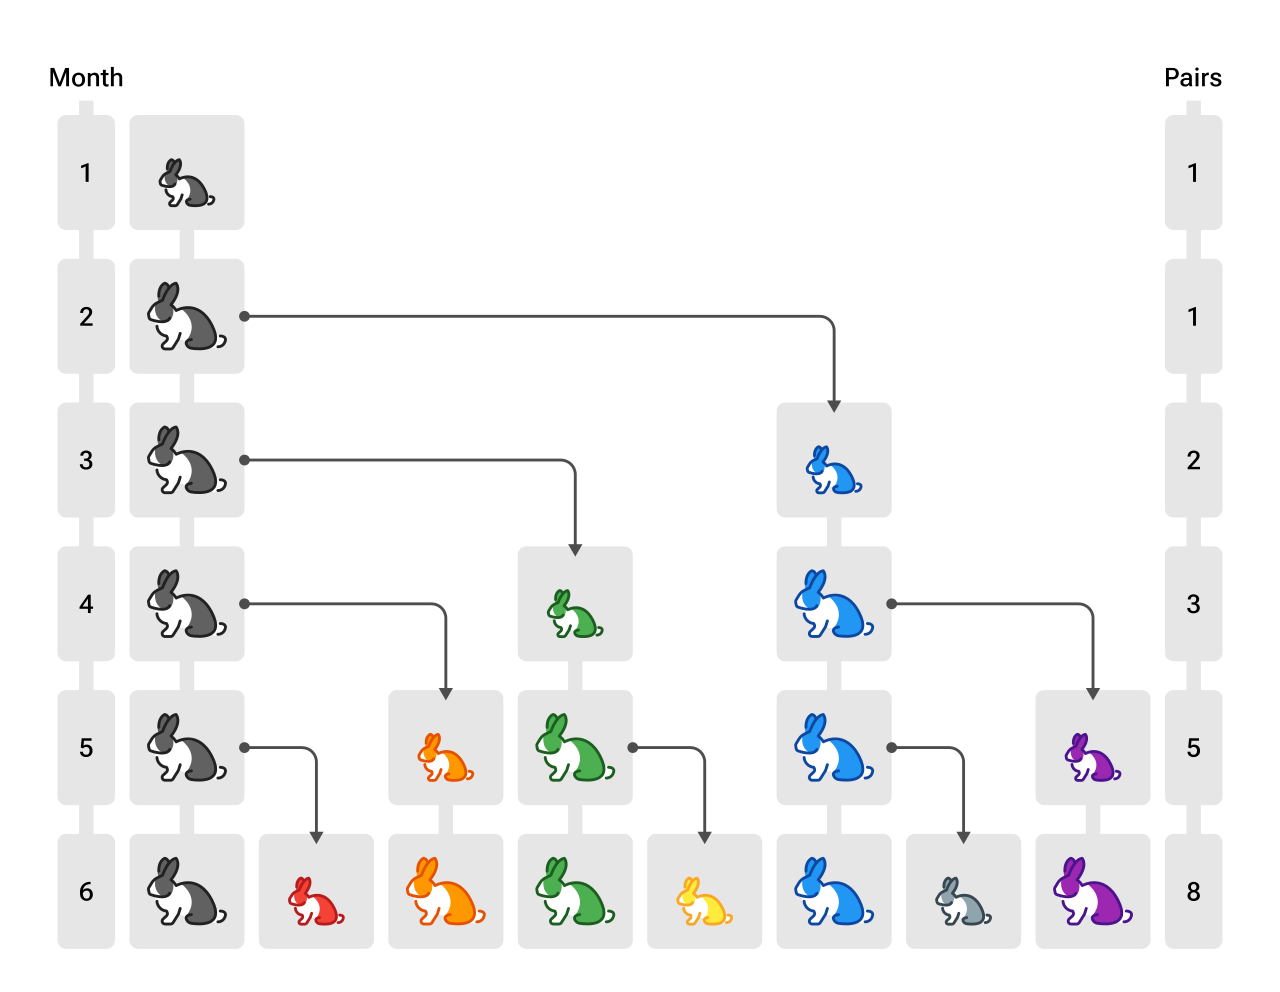
\includegraphics[scale = 0.2]{lesson_1/images/fibonacci_rabbits.png}
\end{center}
\end{frame}

\begin{frame}{Fibonacci sequence}
\small
The problem leads to a series of numbers called the \textbf{Fibonacci sequence}:
\begin{equation*}
1, 1, 2, 3, 5, 8, 13, 21, 34, 55, 89, 144, ...
\end{equation*}
%\pause
The first two numbers are given, and subsequent numbers are found by adding the two numbers before them. Thus, we have the following recursive definition (a recursive definition defines elements in a set in terms of other elements in the set) of Fibonacci numbers:
\begin{align*}
   F_{1} &= F_{2} = 1 \\ 
   F_{n} &= F_{n-1} + F_{n-2}
 \end{align*}
%\pause
The ratio of two consecutive Fibonacci numbers converges to a number known as the \textbf{golden ratio}:
\begin{equation}
  \psi = \frac{1 + \sqrt{5}}{2} \approx 1.618 ...
\end{equation}
\end{frame}

\begin{frame}{Fibonacci sequence}    
A spiral created by drawing circular arcs connecting the opposite corners of squares of A tiling with squares whose side lengths are successive Fibonacci numbers
\vfill

\begin{center}
   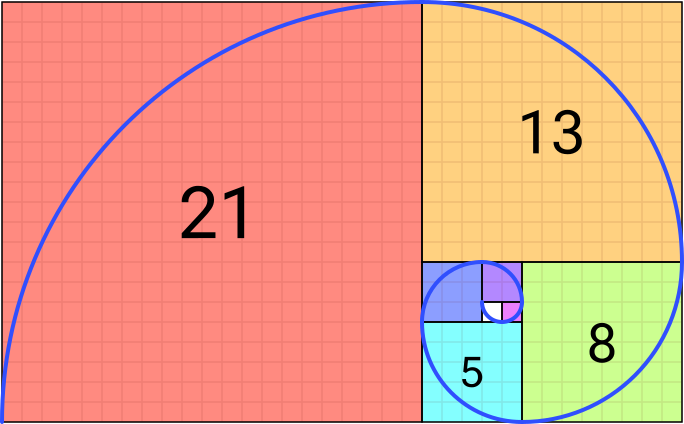
\includegraphics[scale = 0.35]{lesson_1/images/fibonacci_spiral.png} 
\end{center}

\end{frame}


\begin{frame}[t]{Fibonacci sequence in nature}
\footnotesize
\begin{columns}
    \begin{column}{0.6\textwidth}
    \begin{itemize}
    
        \item \textbf{Spiral Patterns}: The growth chambers of a nautilus shell create a distinctive spiral that aproximately follows the Fibonacci sequence and the golden ratio.
        \only<2->{
        \item \textbf{Branches}: Tree branches sometimes follow Fibonacci sequence. Main branch splits into two, then one of those branches splits while the other stays dormant.}
        \only<3->{
        \item \textbf{Flower Petals:} The number of petals on many flowers corresponds to Fibonacci numbers: lilies (3 petals),  buttercups (5 petals), and daisies (often 34 or 55 petals).
        }
        \only<4->{
        \item \textbf{Why?} Fibonacci patterns in nature are likely related to optimal growth and packing efficiency.
        \color{secondary}
        \item \textbf{While the Fibonacci sequence appears  in nature, it is not a universal rule.}
        }
    \end{itemize}
        
    \end{column}
    \begin{column}{0.4\textwidth}
        \only<1>{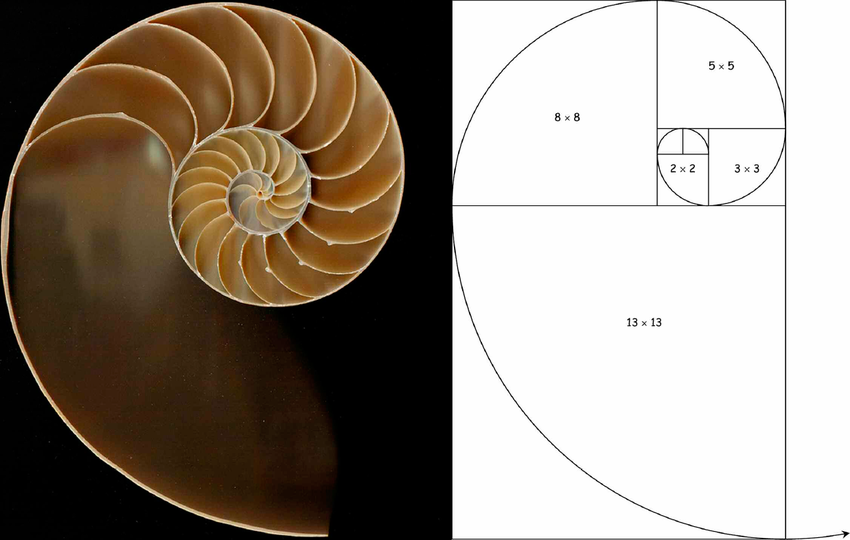
\includegraphics[scale = 0.5]{lesson_1/images/fibonacci_shelll.png}}
        \only<2>{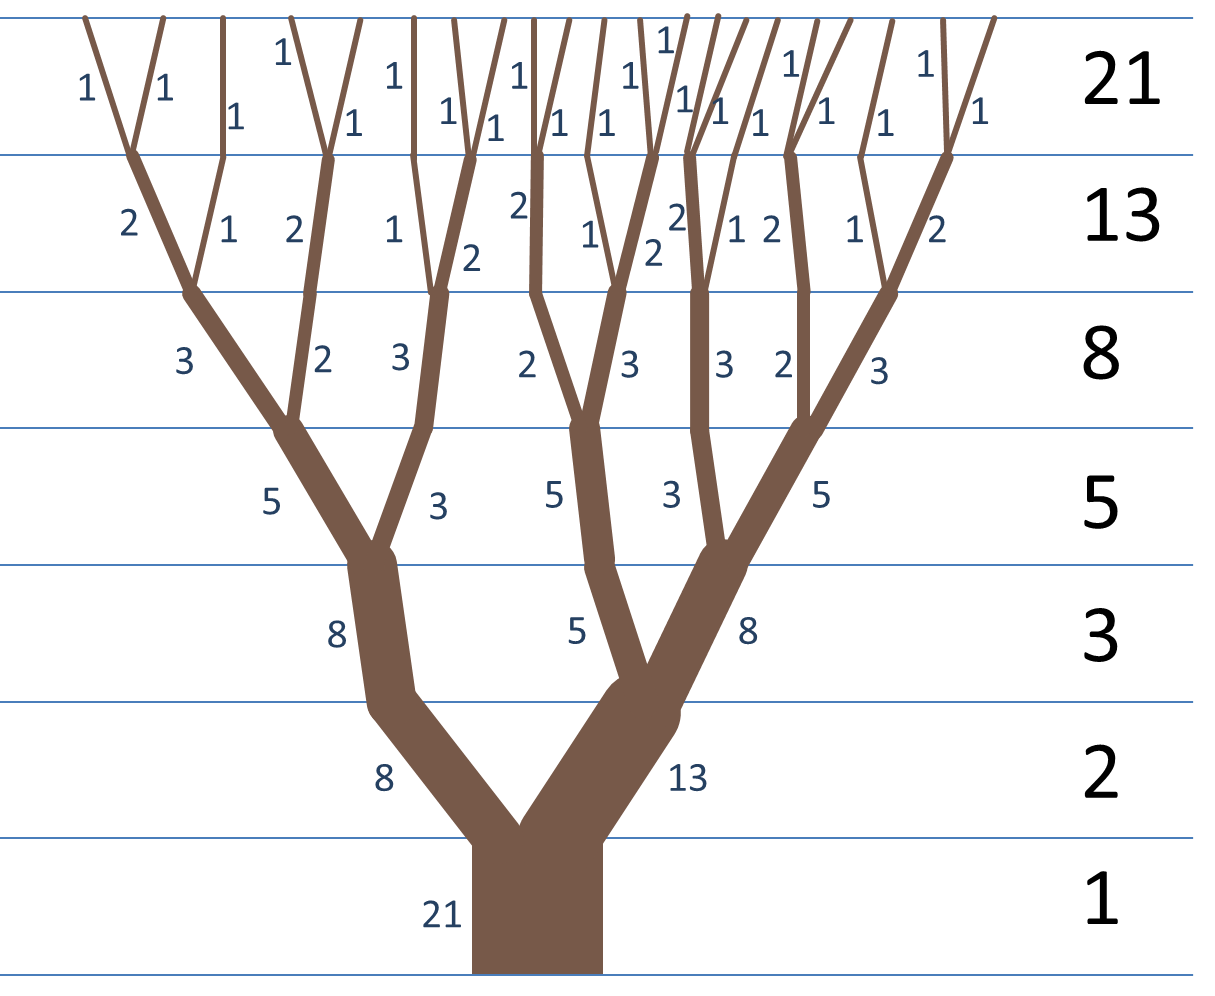
\includegraphics[scale = 0.2]{lesson_1/images/fibonacci_tree.png}}
        \only<3>{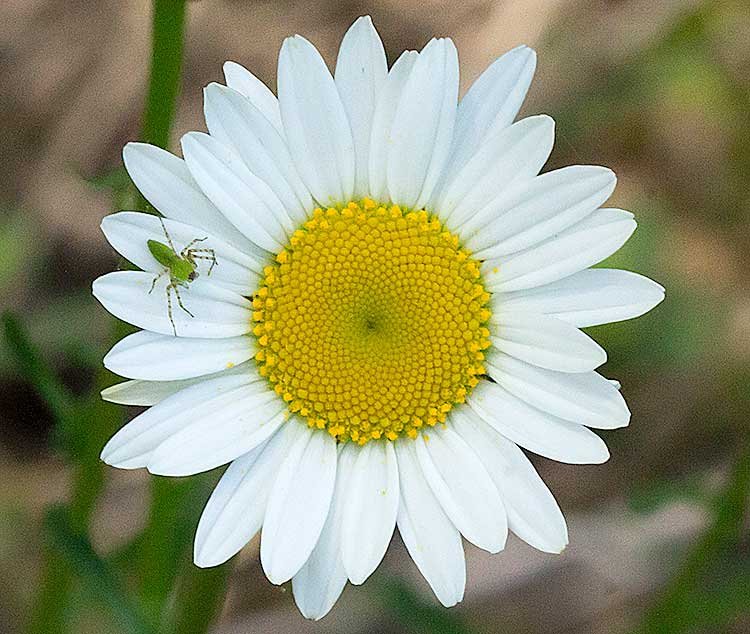
\includegraphics[scale = 0.2]{lesson_1/images/fibonacci_daisy.jpg}}
        \only<4>{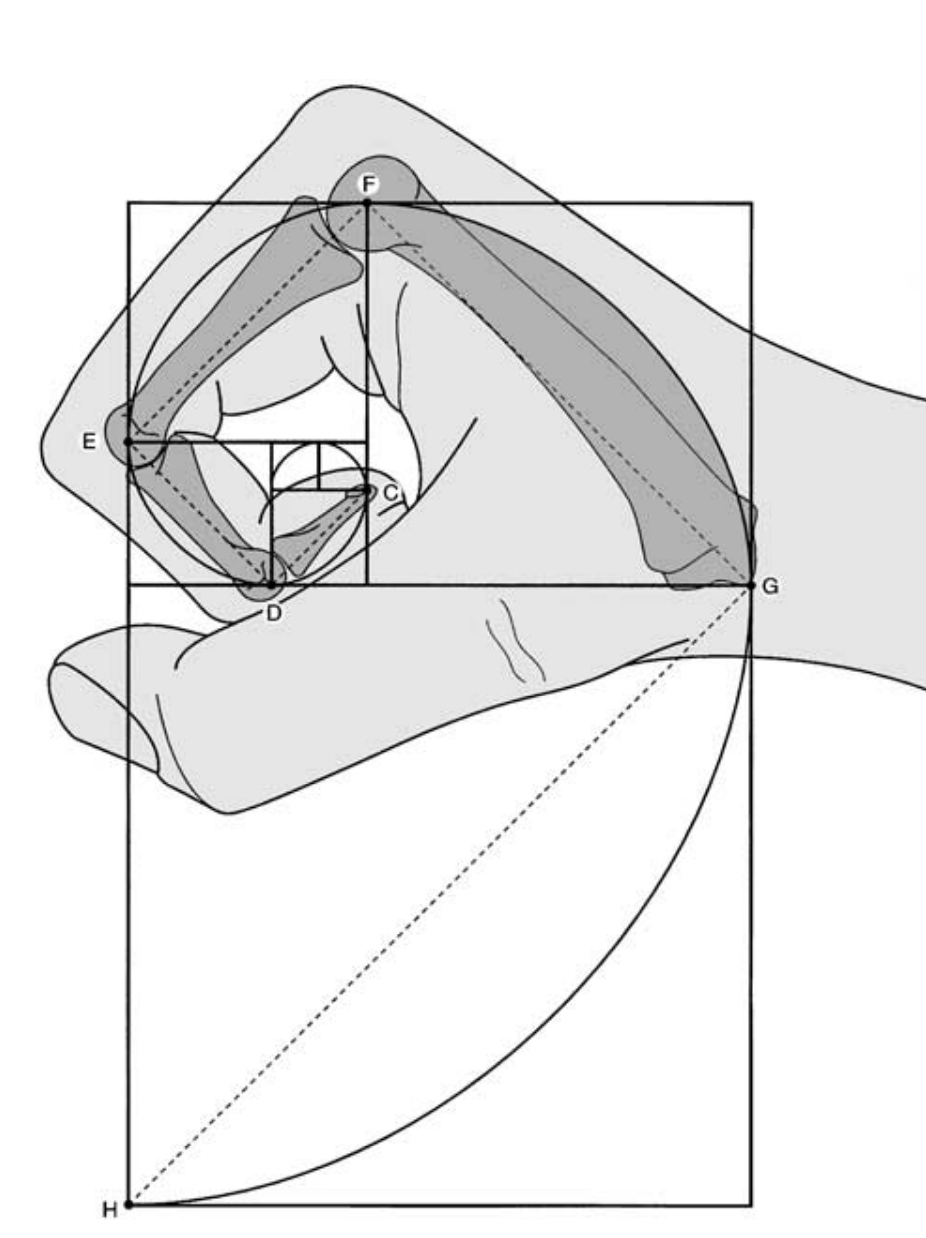
\includegraphics[scale = 0.3]{lesson_1/images/fibonacci_grip.png}}       
    \end{column}
    
\end{columns}
\end{frame}

\begin{frame}{Fibonacci sequence is extensively used in arts}
Golden ratio in famous logos
\begin{center}
    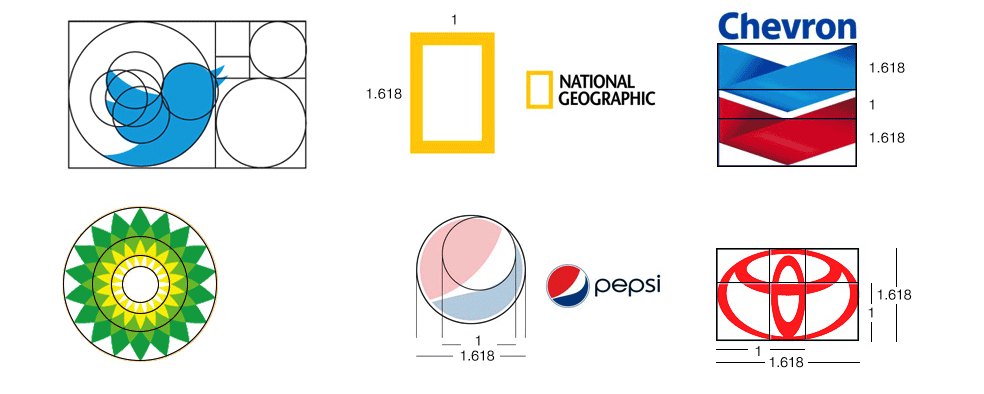
\includegraphics[scale=0.3]{lesson_1/images/fibonacci_logos.png}
\end{center}
\end{frame}



\subsection{Exercise}
\begin{frame}{Fibonacci sequence tasks as  Matlab refresher}
    We will work Fibonacci sequence to go review some basic concepts in Matlab. Basic experience with programming is expected. 
    \vfill
    \textbf{We will cover }
    \begin{itemize}
        \item Loop control statements
        \item Vector and matrix indexing
        \item Functions
        \item Plotting
    \end{itemize}
\end{frame}


\begin{frame}{Task 1.1: Loop control statements}
With loop control statements, you can repeatedly execute a block of code. There are two types of loops:
\begin{enumerate}
    \item \textbf{for} statements loop a specific number of times, and keep track of each iteration with an incrementing index variable.
    \item \textbf{while} statements loop as long as a condition remains true.
\end{enumerate}

Your tasks: 
 \begin{enumerate}
     \item  Generate first 20 elements of Fibonacci sequence with help of for loop
     \item  Generate all number of Fibonacci sequence smaller than 500 using while loop
 \end{enumerate}
 \textit{Note: Save generated numbers to a vector, we will need them for the next task}
\end{frame}


\begin{frame}[fragile]{Solution 1.1.1: First 20 Fibonacci numbers } 
Generate first 20 elements of Fibonacci sequence using \textbf{for} loop
\vfill
\small
\lstinputlisting{lesson_1/code/task_1_1_1_fibonacci_for_loop.m}
\end{frame}

\begin{frame}[fragile]{Solution 1.1.2: Fibonacci numbers smaller than 500} 
Generate all number of Fibonacci sequence smaller than 5000 using \textbf{while} loop
\vfill
\small
\lstinputlisting{lesson_1/code/task_1_1_2_fibonacci_while_loop.m}
\end{frame}

\begin{frame}{Task 1.2: Vector Indexing}
Vector indexing allows you to access and manipulate specific elements within a vector.  Here are the most common techniques:
\vspace{1em}

\begin{itemize}
    \item \textbf{Linear Indexing}
    \begin{itemize}
        \item Access elements by their position in the vector: \lstinline{x(3)} gets the third element of x; \lstinline{x(end)} the last element.
        \item Use ranges with the colon operator:  \lstinline{x(2:5)} gets elements 2 to 5 of vector x
    \end{itemize}
    \item \textbf{Logical Indexing}:

    \begin{itemize}
        \item Create a logical array the same size as your vector to get elements where the condition is true: \lstinline{x(x > 10)} extracts elements greater than 10).
    \end{itemize}
\end{itemize}
\end{frame}

\begin{frame}{Task 1.2: Vector Indexing}
\textbf{Your tasks}
\begin{itemize}
    \item Divide 6\textsuperscript{th} and 5\textsuperscript{th} element of vector with Fibonacci numbers. 
    \item Divide last and 2nd last element of vector with Fibonacci numbers. 
    \item Get all Fibonacci numbers smaller than 50 
     \item Get all Fibonacci numbers between 50 and 500
    \item With help of indexing and \lstinline{mod} function replace all even Fibonacci numbers in the vector with 0.
\end{itemize}
\end{frame}

\begin{frame}{Task 1.2: Solution}
\begin{itemize}
    \item Divide 6\textsuperscript{th} and 5\textsuperscript{th} element of vector with Fibonacci numbers.
    %\pause
    \newline \lstinline{fib\_seq(6) / fib\_seq(5)}
    %\pause
    \item Divide last and 2nd last element of vector with Fibonacci numbers. 
    %\pause
    \newline \lstinline{fib\_seq(end) / fib\_seq(end-1)}
    %\pause
    \item Get all Fibonacci numbers smaller than 50 
    %\pause
    \newline \lstinline{fib_seq(fib_seq < 50)}
    %\pause
     \item Get all Fibonacci numbers between 50 and 500
    %\pause
    \newline \lstinline{fib_seq(fib_seq > 50 & fib_seq < 500)}
    %\pause
    \item With help of indexing and \lstinline{mod} function replace all even Fibonacci numbers in the vector with 0.
    %\pause
    \newline \lstinline{fib_seq(mod(fib_seq,2) ~= 0) = 0}
\end{itemize}
\end{frame}

\begin{frame}{Matrix indexing is similar to vector indexing}
\small
\begin{itemize}
    \item Define matrix
    \newline \lstinline{M = [1,2,3; 4,5,6; 7,8,9]}
    \item Extract the element in row 2, column 3
    \newline \lstinline{M(2,3)}
    One or both of the row and column subscripts can be vectors:
    \newline \lstinline{M(1:3,2:3)}
    \item A  "\lstinline{:}"  is shorthand notation for 1:end 
    \newline \lstinline{M(:,2:3)}
    \item When put one subscript, MATLAB treats M as if its elements were strung out in a long column.
    \newline \lstinline{M(8)}
    \item You use a logical array as subscript. MATLAB extracts true elements in the form of a column vector
    \newline \lstinline{N = [1.3, 2.0, 3.8; 4.8, 5.0, 6.0]}
    \newline \lstinline{N(mod(N,1) = 0)} 
    \newline \lstinline{N(N>3)}
\end{itemize}
\end{frame}


\begin{frame}[fragile]{Task 1.3: Functions background }
\begin{itemize}
    \item Functions are reusable blocks of code that take inputs, perform calculations, and return outputs. They are essential for code organization and modularity. 
    \item Functions in Matlab can be defined in a separate script or at the end of a script file 
\end{itemize}
    
\begin{lstlisting}
% call function
my_circile = circle_area(5)

% declare function
function area = circle_area(radius)
    pi = 3.14159; % approx. value of pi
    area = pi * radius^2; 
end
\end{lstlisting}
\end{frame}

\begin{frame}{Task 1.3: Functions}
\textbf{Your task}
\begin{enumerate}
    \item Writer function to return vector with generated \textit{n} Fibonacci numbers
    \item Write function to return random Fibonacci number 
    \item Check if the number is Fibonacci 
\end{enumerate}
\vspace{1em}
\textit{Think about your solution fist; after that fell free to search for hints online.}   
\end{frame}

\begin{frame}[fragile]{Solution 1.3.1: Fibonacci generator}
\small
\begin{itemize}
    \item We will reuse our previous Task 1.1 code.
    \item  The subsetting is important for n values 1 or 2. 
    \item \textbf{What are limitation of this code?}
\end{itemize}

\vfill
\lstinputlisting{lesson_1/code/task_1_3_1_fibonacci_generator.m}

\end{frame}

\begin{frame}[fragile]{Solution 1.3.2: Random Fibonacci number}
\footnotesize
\lstinputlisting{lesson_1/code/task_1_3_2_random_fibonacci.m}
\end{frame}

\begin{frame}[fragile]{Solution 1.3.3: Check if number is Fibonacci}
One possible approach : Check if the last generated number before overstepping treshold is Fibonacci number.
\footnotesize
\lstinputlisting{lesson_1/code/task_1_3_3_fibonacci_check.m}   
\end{frame}

\begin{frame}{Task 4: Plotting}
Plotting allows you to represent your data graphically, which is always a good idea. MATLAB offers a wide range of plots. Here we cover only basic line plot.

Your tasks: 
 \begin{enumerate}
     \item  Plot the first 15 elements of Fibonacci sequence
     \item  Calculate and plot ratio of all \lstinline{n(i+1)/n(i)} in the first 15 elements of Fibonacci sequence.  
 \end{enumerate}
\end{frame}

\begin{frame}[fragile]{Solutions 1.4}

\small
1. Plot the first 15 elements of Fibonacci sequence:
\lstinputlisting[firstline=9,lastline=10]{lesson_1/code/task_1_4_fibonacci_plot.m}
\vfill
2. Calculate and plot ratio of all \lstinline{n(i+1)/n(i)} in the first 15 elements of Fibonacci sequence. 
\lstinputlisting[firstline=12]{lesson_1/code/task_1_4_fibonacci_plot.m}
\vfill
\textit{Note: Period "." signifies element-wise operation}
\end{frame}
